\chapter{Architecture and Design}

This chapter's aim is to familiarize the user with the design decisions and the
architecture of the application, describe the challeenges encountered during
development and provide solutions to some of them.

%----------------------------------------------------------------------------
\section{Architecture}\label{sec:Architecture}
%----------------------------------------------------------------------------

The application's components can be separated into three main categories:

\begin{itemize}
  \item Java-Compile Time - components that are used while designing the
  queries and generating code.
  \item \CPP{} Compile Time - the generated code.
  \item \CPP{} Runtime - the code running the queries.
\end{itemize}

The architecture of the application is shown on figure \figref{architecture}.
The main component of the architecture is the ECore model, which serves as
the description of the possible object types and their relationships.
In my case this is basically similar to an UML class diagram. Further
detail will be discussed in chapter \sectref{CppObjectModel}.

\begin{figure}[!ht]
\centering
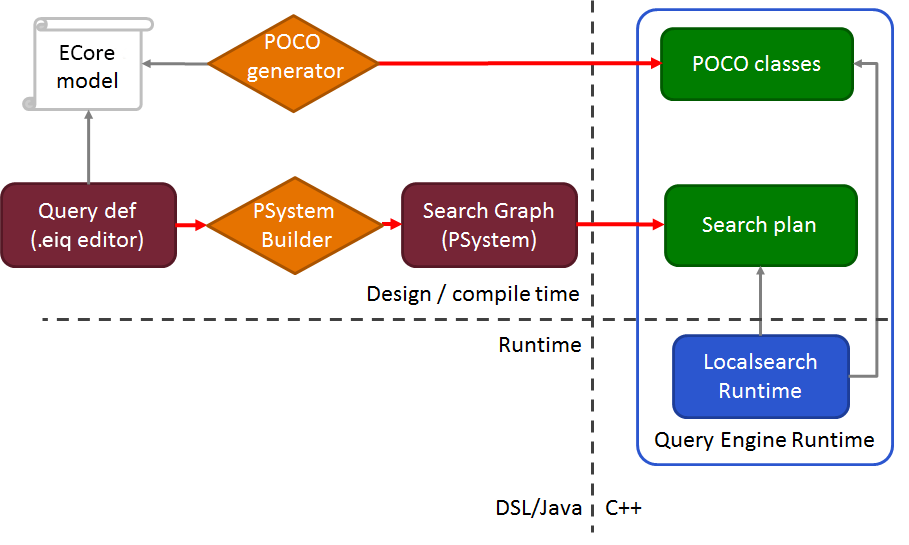
\includegraphics[width=150mm, keepaspectratio]{figures/architecture.png}
\caption{The architecture of the engine}
\label{fig:architecture}
\end{figure}

From the ECore model, the POCO generator (\sectref{GeneratedCodeStructure})
generates the \CPP{} classes. These are the classes the runtime model consists
of and the queries can be executed on.

Writing queries is supported through the \EIQ{} pattern language editor, which
provides content assist, syntax highlighting, validation and several other
features to help the user in query development.

From the query definition the search graph (called \emph{PSystem} in
\EIQ{}) gets transformed. This search graph contains every information
necessary to create the search plan. The search plan gets transformed from the
search graph to Java first, then based on this plan the actual search operations
get transformed into \CPP{} code. The available search operations and their
execution is coded in a runtime library. The assembly of the actual search plan
and its execution gets obfuscated by generated code, the user only has to call
the appropriate generated method to get the matching elements to a specific query.

This architecture makes it so that the user has no interaction with any
localsearch related part of the application, i.e. he has to create the model,
write the queries and later on call the queries in his \CPP{} application,
everything else is handled hidden from him.

\section{EMF to \CPP{} generation} \label{sect:CppObjectModel}

This section focuses on the ECore metamodel used to describe the class hierarchy
of the generated code and the structure of the generated code.

%----------------------------------------------------------------------------
\subsection{Metamodel}\label{sec:Metamodel}
%----------------------------------------------------------------------------

\begin{figure}[!ht]
\centering
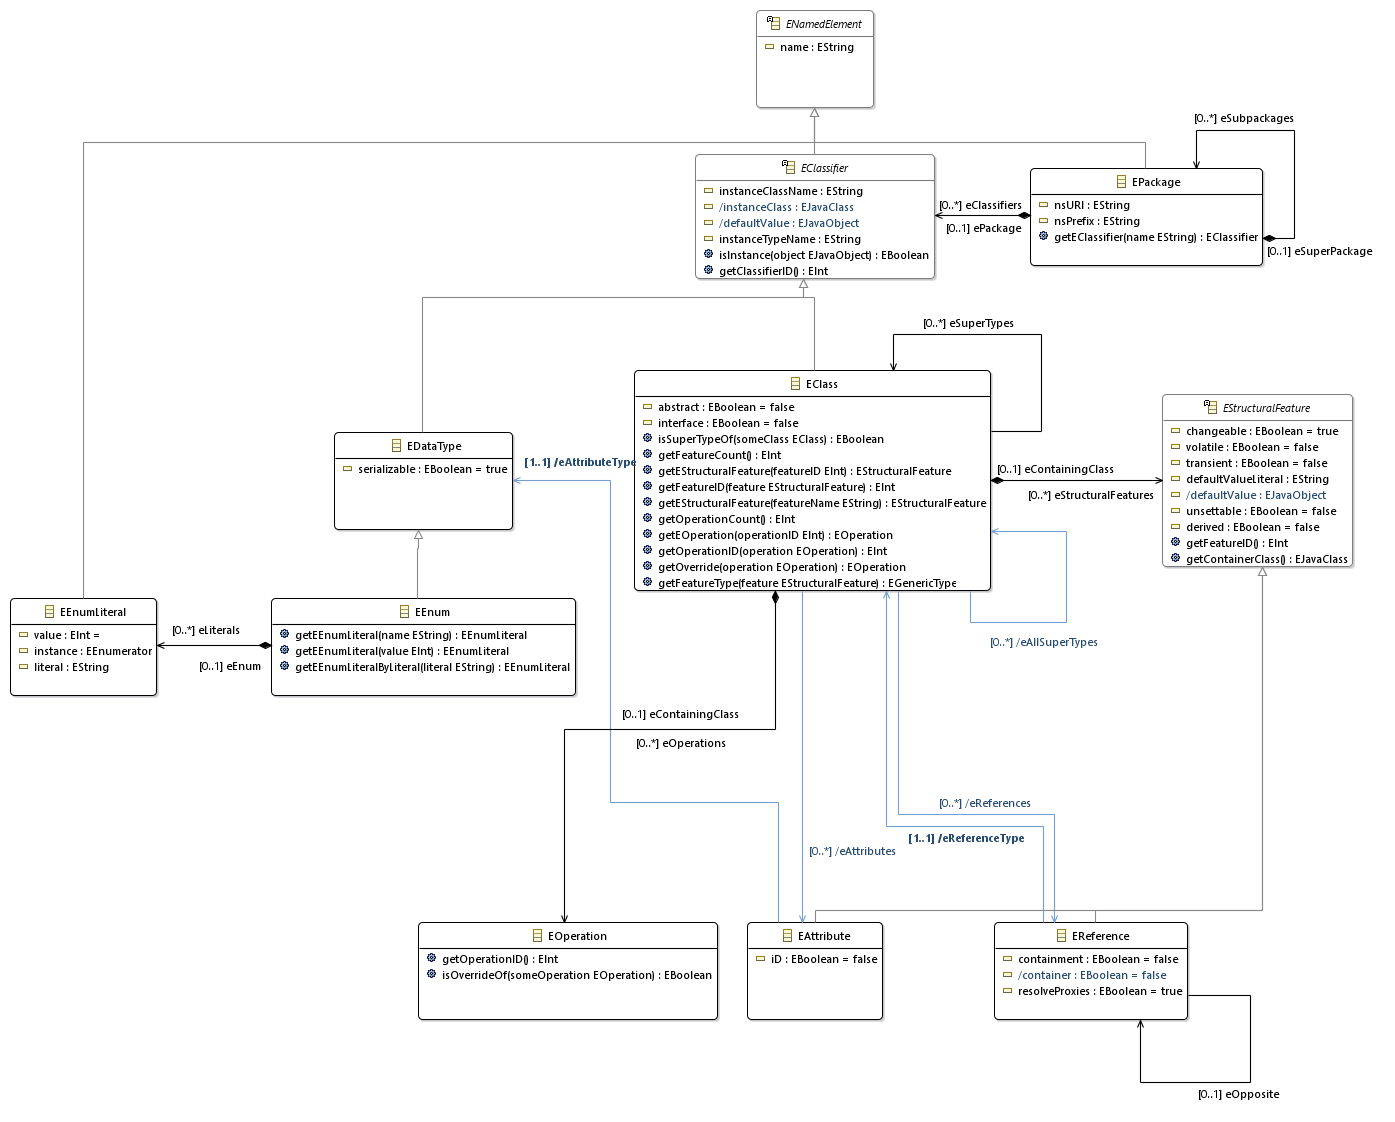
\includegraphics[width=160mm, keepaspectratio]{figures/ecore_diagram.png}
\caption{The ECore Class diagram metamodel}
\label{fig:metamodel}
\end{figure}

The metamodel (as seen on figure \figref{metamodel}) is a simplified version of
the ECore metamodel. Ecore is a reference implementation of OMG's MOF
standard. It allows expressing other models while it is its own metamodel,
meaning ECore is defined using its own concepts. The root of ECore is
\emph{EPackage}, which is a simple container for organization purposes. It
may contain other EPackages or \emph{EClassifiers}, which can either
be an \emph{EClass} or an \emph{EDataType}. An EDataType are primitive types
like integer, string or enum, which corresponds to \emph{EEnum}. An EEnum may
contain multiple literals represented by \emph{EEnumLiteral}. An EClass serve as
a class in object oriented programming (OOP). It can be a regular class, an
abstract class or an interface, corresponding to the respective meaning in OOP.
An EClass contains EStructuralFeatures. An EStructuralFeature may either be an
\emph{EReference}, an \emph{EAttribute} or an \emph{EOperation}. An EReference
is an association between two EClasses, which may be a containment reference
meaning the source of the reference contains the value of the actual object or
objects referenced. Each EReference may possess an \emph{eOpposite} if there is
an EReference in the opposite direction. An EAttribute represents a simple
primitive type attribute for a EClass, like an integer, string, boolean etc. An
EOperation corresponds to a function declaration. Defining a function is not
directly supported by the metamodel.

%----------------------------------------------------------------------------
\subsection{Generated code structure}\label{sect:GeneratedCodeStructure}
%----------------------------------------------------------------------------

To talk about the generated code structure, it is necessary to have an actual
model to generate the code from. For this purpose, I used the previously
introduced school model shown on figure \figref{School_Metamodel}. The structure
of the generated code can be seen on figure \figref{GenCodeStruct}.

\begin{figure}[!ht]
\centering
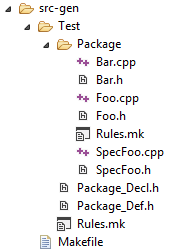
\includegraphics[width=40mm, keepaspectratio]{figures/gen_code_struct.png}
\caption{The generated code structure}
\label{fig:GenCodeStruct}
\end{figure}

The model school got generated into a folder named accordingly inside the
cpp-gen folder of the project. For every EPackage  a folder and two header files
are created. The header file postfixed with \emph{def} contains includes to
the definition of the classes inside the package, while the one postfixed with
\emph{decl} contains the declaration of said classes. The folder created for the
package contains header and source files for each EClass and, if there are any,
the above explained files for contained EPackages. To help with compilation, a
makefile also gets generated. The root model folder has the makefile itself,
which then includes the rule files in the folders recursively. This way the
users only job is to create the main file and the code can be easily compiled.
Another way to use the generated code would be to simply include the rule file
in the user's own makefile in another project. This gives great flexibility to
anyone using a make based build tool.

\section{Runtime Library}

This section will mostly focus on the implementation specific details of the
\CPP{} local search runtime, such as problems specific to \CPP{} and their
solutions, the structure of a search plan, its operations and their execution.

%----------------------------------------------------------------------------
\subsection{\CPP{} specific problems}\label{sect:CppSpecificProblems}
%----------------------------------------------------------------------------

In the case of the runtime, \CPP{} brought with its speed several problems, such
as the lack of any reflection API and a unified object base class. This caused
several issues during the implementation, because running local search over \CPP{}
objects requires instance checking, getting fields by name to navigate
associations and iterating over every instance of a specific task. This section
will propose a solution for each of the above mentioned issues.

%----------------------------------------------------------------------------
\subsubsection{Objects in \CPP{}}\label{sect:ObjectsInCpp}
%----------------------------------------------------------------------------

During the local search process it is necessary to hold every single object in
containers without knowing their type. In \CPP{} there are three main ways to do
this.

\begin{itemize}
  \item using heterogeneous collections with a common base class
  \item \emph{void*} pointer
  \item wrapper object
  \item using templates
\end{itemize}

Using a common base class is probably the easiest and most obvious solution,
but it would constraints the type of objects the local search runtime can
be used on which makes this solution undesirable.

Using \emph{void*} pointers would mean the complete loss of type information,
thus making any dynamic type checking mostly impossible. This alone makes this
solution unusable.

The third method of using wrapper object is a possible solution with the
only drawbacks of being complicated, slow and memory inefficient.

The last, template based version is probably the most complicated one. It
requires complicated template programming which results in slower compile times
and larger executables, but it has a superior runtime speed and memory usage to
all other alternatives.

\textbf{Wrapper object based solution}

 The structure of the wrapper object can be seen on figure
 \ref{fig:wrapper_structure}.

\begin{figure}[!ht]
\centering
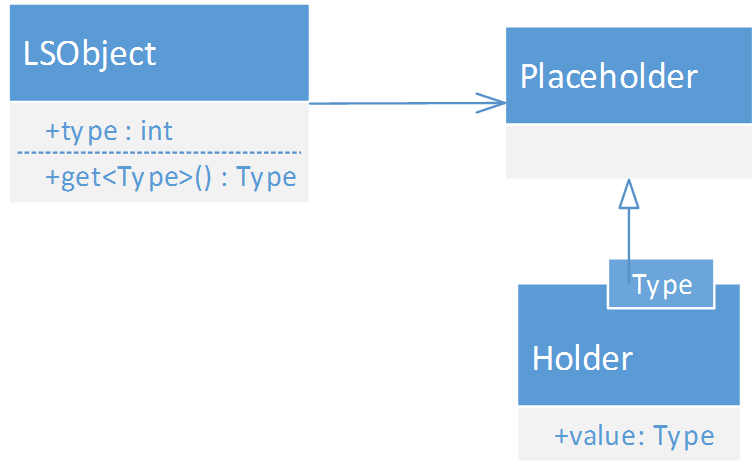
\includegraphics[width=70mm, keepaspectratio]{figures/wrapper_structure.png}
\caption{The structure of the wrapper object}
\label{fig:wrapper_structure}
\end{figure}

The \emph{LSObject} (Local Search Object) contains the type information, a
template method to get the value contained cast to the proper type and a pointer to a
\emph{Placeholder} object. The actual object contained is actually of the
\emph{Holder} template type, which contains the original value. The placeholder
object's construction can be seen as below.

\begin{lstlisting}[frame=single,float=!ht,language=C++, caption=Constructing a
wrapper object] template<typename T>
LSObject(const T& value, int type) :
	_ptr(new Holder<T>(value)), type(type) {
}
\end{lstlisting}

As it can be seen from the code, the \emph{LSObject}'s holder will hold a
reference to the value, be it pointer or actual value. The second parameter
\emph{type} contains the type information for the value. 

\begin{lstlisting}[frame=single,float=!ht,language=C++, caption=Retrieving
correctly typed object]
template<typename T>
inline T& LSObject::get() const {
    return static_cast<Holder<T>&>(*this->_ptr).value;
}
\end{lstlisting}


The \emph{get} method of the wrapper object returns the value as it was passed
in, however this require the compile time knowledge of the original type. The
implementation can be seen below:

The usage of the wrapper class is shown in listing \listref{wrapper_usage}.

\begin{lstlisting}[frame=single,float=!ht,language=C++,
label=listing:wrapper_usage, caption=Wrapper object usage]
Foo f;
f.Name = "Foo1";
LSObject ls_f(f, 0);

ls_f.get<Foo>().Name
\end{lstlisting}

The design of the class was heavily inspired by the
\emph{boost::any}\cite{boost-any} class.

The main problem with this approach is its speed. The speed issue is caused by
the fact that while iterating over the instances of a class, they all have to be
wrapped in a wrapper class while creating a new collection. This costs a
considerable amount of time. Also for this reason, the memory footprint of this
solution is considerably higher.

\textbf{Template based solution}

This solution needed the most effort in implementation, since this requires
the type information to flow through the whole runtime. The main idea of the
solution is that all components of the engine have several template parameters
to describe the types it has to handle. The listing \listref{template_example}
contains the declaration of a navigation class, which shows how complicated
class declarations can get using this approach.

\begin{lstlisting}[frame=single,float=!ht,language=C++,
label=listing:template_example, caption=Template based approach example]
template<typename SrcType, typename TrgType, typename Collection, 
		typename Member, typename MatchingFrame>
class NavigateMultiAssociation
  : public ExtendOperation<TrgType, Collection, MatchingFrame>;
\end{lstlisting}

The main benefits of this solution are speed and really low memory usage. The
speed is gained from the fact that, with this approach, iterators can be used
over the original instances collections without any wrapping, and only
filtering is necessary. This also means that the memory usage scales with
pattern complexity and is completely independent of model size.

%----------------------------------------------------------------------------
\subsubsection{Iterating class instances}\label{sect:IteratingClassInstances}
%----------------------------------------------------------------------------

To allow iteration over all instances of a class, a registry needs to be managed
which gets updated on each instance construction or deletion. The only feasible
way to do this is to write the classes constructor and destructor in a way that
it adds new instances to a list when they are created and removes them when they
are deleted. This method limits the type of objects the runtime works on, but
this is the most reasonable solution. An example of a class prepared to count
its instances can be seen below.

\begin{lstlisting}[frame=single,float=!ht,language=C++]
class Foo  {
public:
	Foo() {
		_instances.push_back(this);
	}
	
	~Foo() {
		_instances.remove(this);
	}
		
	static std::list<Foo*> _instances;
};
\end{lstlisting}

This solution uses the \emph{std::vector} to contain the created instances.
While the constructor is trivial the destructor is more interesting. The
check whether the destructed object is in the vector seems unnecessary, but \CPP{}
allows the allocation of memory for an object without actually calling its
constructor. This memory portion can be freed with delete which also calls the
destructor. In this case, the instance will not be in the vector and this could
cause issues.

%----------------------------------------------------------------------------
\subsubsection{Instance checking}\label{sect:InstanceChecking}
%----------------------------------------------------------------------------

In the case of \CPP{} the generally accepted way of dynamic type checking is using
\emph{dynamic\textunderscore cast} provided by the language. This is however a
not ideal solution. The first problem is it only works on dynamic classes, i.e.\
classes with at least one virtual method. The other issue is speed, as
\emph{dynamic\textunderscore cast} uses vtables to check if the specified
instance can be casted to the specified type. To illustrate the speed issues,
the following table (\ref{tab:InstPerf}) shows the results of performance tests
made in \CPP{} and Java.

\begin{table}[ht]
	\footnotesize
	\centering
	\caption{Instance of check performance comparison of Java and \CPP{}}\label{tab:InstPerf}
	\begin{tabular}{ | l | c | c |}
	\hline
	Iterations 	& Java 		& \CPP{} 		 \\ \hline
	$10^4$ 		&  1	ms 	& 0.1	ms \\
	$10^5$ 		&  11 	ms  & 1		ms \\
	$10^6$ 		&  15 	ms  & 17	ms \\
	$10^7$ 		&  41 	ms  & 173	ms \\
	$10^8$ 		&  261 	ms  & 1746	ms \\
	$10^9$ 		&  2515 ms  & 17456	ms \\
	\hline
	\end{tabular}
	\label{tab:TabularExample}
\end{table}

As the table shows, Java is slower on small number of iterations, but on higher
number of iterations the JIT compiler manages to optimize the instance checking
process and gets roughly a magnitude faster than \CPP{}.

The solution I propose is an inheritance matrix in which it is contained whether
an instance of a type is a child of another type. This can be generated using
the model of the classes. This also means that most of the calculation is done
generation time, thus making this method faster than most dynamic type
inference method provided by languages. For the following examples I will use
the class structure shown on figure \ref{fig:simple_class} . In this example
there are three classes, \emph{Foo}, \emph{Bar} and \emph{SpecFoo}.
\emph{SpecFoo} extends \emph{Foo}. The example does not contain any of
the possible more complex hierarchy structures, like diamond, but nonetheless it
supports them.

\begin{figure}[!ht]
\centering
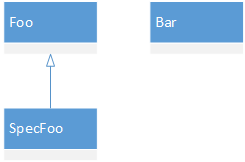
\includegraphics[width=50mm, keepaspectratio]{figures/simple_class.png}
\caption{Example class structure}
\label{fig:simple_class}
\end{figure}

To use this method, the runtime knowledge of a classes exact instance is
required. This could be done via a virtual method (which is undesirable
because of larger memory footprint for instances) or template metaprogramming.
Template metaprogramming would only work on the static type of the object, not
the dynamic, i.e. it would not work correctly with inheritance. For example for
the pointer \emph{Foo* f = new SpecFoo()} it would always return Foo as the
type, same with the built in \emph{\texttt{type\_id}} function. Thus the only
viable solution in my case is the virtual method. An implementation example for
such solution can be seen in the following example (expanding upon the
previous code sample):

\begin{lstlisting}[frame=single,language=C++, label=listing:type_id,
caption=Type identifier for classes]
class Foo  {
public:
	Foo() {
		_instances.push_back(this);
	}
	
	~Foo() {
		_instances.remove(this);
	}
	
	virtual unsigned short get_type_id() const {
        return type_id;
    }
		
	static std::list<Foo*> _instances;
	static const unsigned short type_id = 1;
};
\end{lstlisting}

In this example, the \emph{\texttt{type\_id}} is generated. This might cause
issues if the code is generated in multiple sessions. This can be solved with a
class that has a growing id for each of its instance, and a bit of template
metaprogramming. A simplified solution can be seen in listing
\listref{unique_number}.

\begin{lstlisting}[frame=single,float=!ht,language=C++,
label=listing:unique_number, caption=Unique number generation for type
identifiers]
class unique_number { 
public:
	unique_number(): cur_id(max_id++) {}

private:
	static unsigned long max_id;
	unsigned long cur_id;
};

template<typename C>
struct type_number {
	static unique_number number;
};

class Foo  {
	...
	virtual unsigned short get_type_id() const {
        return type_number<Foo>::number;
    }
	...
};
\end{lstlisting}

The basic idea is that every instance of \emph{\texttt{unique\_number}} contains
a unique identifier. For each class, a separate \emph{\texttt{type\_number}}
gets created compile time with a \emph{\texttt{unique\_number}} inside, which can be
retrieved in the \emph{\texttt{get\_type\_id}} method. This guarantees a unique
id for each class that's calculated compile time.

Using this type id as an identifier it is possible to create a boolean matrix
(two dimensional array) of the type relationships. For each member of this matrix
'm' 
\[
m[type1][type2] = type1\textrm{ instanceof }type2
\]

In the case of the presented example this matrix would look like in the
following table (\ref{tab:InhMatrix}):

\begin{table}[ht]
	\footnotesize
	\centering
	\caption{Example inheritance matrix}\label{tab:InhMatrix}
	\begin{tabular}{| c | c | c | c |}
	\hline
			& Foo	& Bar	& SpecFoo	\\ \hline
	Foo		& true	& false	& false		\\ \hline
	Bar		& false	& true	& false		\\ \hline
	SpecFoo	& true	& false	& true		\\ \hline
	
	\hline
	\end{tabular}
	\label{tab:TabularExample}
\end{table}

The diagonal of the matrix is obviously true (since an instance of Foo is
trivially the instance of Foo). The SpecFoo instance is the instance of both Foo
and SpecFoo.

This method allows instance checking to be done in basically two array indexing
operations. From my performance measurements, this method seem to be marginally
faster than the Java \emph{instanceof} operation.

\begin{table}[ht]
	\footnotesize
	\centering
	\caption{Instance of check performance comparison of Java,
	\CPP{} and inheritance matrix}\label{tab:InstPerf}
	\begin{tabular}{ | l | c | c | c |}
	\hline
	Iterations 	& Java 		& \CPP{}	&	Inheritance Matrix	\\ \hline
	$10^4$ 		&  1	ms 	& 0.1	ms	&	0.03	ms			\\
	$10^5$ 		&  11 	ms  & 1		ms	&	0.3		ms			\\
	$10^6$ 		&  15 	ms  & 17	ms	&	3		ms			\\
	$10^7$ 		&  41 	ms  & 173	ms	&	15		ms			\\
	$10^8$ 		&  261 	ms  & 1746	ms	&	172		ms			\\
	$10^9$ 		&  2515 ms  & 17456	ms	&	1725	ms			\\
	\hline
	\end{tabular}
	\label{tab:TabularExample}
\end{table}

%----------------------------------------------------------------------------
\subsubsection{Navigation through associations}
\label{sect:NavigationThroughAssociations}
%----------------------------------------------------------------------------

Navigation through associations specified by their name requires meta
information about the classes. This information can be accessed using the \CPP{}
feature called \emph{pointer to member}. A pointer to member is similar to a
function pointer in that they allow the calling of a member function without
knowing its name. Yet, unlike ordinary an ordinary pointer to function, it also
enables the manipulation of data members of an object.

The following listing (\listref{p2m_decl}) shows an example of a pointer to
member declaration. In this case, a pointer to a member of the \emph{Teacher}
class is declared, which member has a \emph{std::string} type.

\begin{lstlisting}[frame=single,float=!ht,language=C++,
label=listing:p2m_decl, caption=Pointer to member declaration]
std::string Teacher::*name;
\end{lstlisting}

A pointer to member can be initialized to any member of the declared class with
the declared type. Listing \listref{p2m_init} shows how to do so.

\begin{lstlisting}[frame=single,float=!ht,language=C++,
label=listing:p2m_init, caption=Pointer to member initialization]
std::string Teacher::*name = &Teacher::name;
\end{lstlisting}

This pointer to member can be passed around to functions as parameter. With
this, it is easy to implement a simple method which navigates over an
association for any class. An example of such a method is shown in listing
\listref{p2m_usage}.

\begin{lstlisting}[frame=single,float=!ht,language=C++,
label=listing:p2m_usage, caption=An universal navigation method using pointer
to member] 
template<SrcType, TrgType, Member>
TrgType navigate(SrcType src, TrgType Member::* navigator) {
  return src->*navigator;
}
\end{lstlisting}

In this example, it is assumed that \emph{Member} and \emph{SrcType} is the
same. In a more realistic use case, the variable \emph{src} has to be casted to
either \emph{Member} or \emph{Member*} depending on weather \emph{SrcType} was a
pointer or value (which can be determined through template metaprogramming).

%----------------------------------------------------------------------------
\subsubsection{Missing value representation}
\label{sect:MissingValueRepresentation}
%----------------------------------------------------------------------------

The query APIi uses Match class instances to represent the query results. These
classes are basically tuples which contain all the data related to a query
result. As the API supports querying of a single arbitrary match, it is
necessary to represent a missing value. This could be done using nullptr, but
that would require the result object to be a pointer, which means it has to be
dynamically allocated on the memory. This should be avoided, so another solution
was necessary.

The most common approach of representing a missing value is the null object
pattern. For this purpose, the runtime library contains an \emph{Optional}
class, which represents either a value or the absence of a value.

Listing \listref{optional} shows the interface of the optional class. An
optional instance can be requested through static methods, for either a missing
value or a present value. The \emph{get} method allows the retrieval of the
value or throws an error if the value is missing. It is possible to check for
the presence of a value through the \emph{present} method. There are additional
utility methods to handle the presence or absence of a value in a functional
style.

\begin{lstlisting}[frame=single,float=!ht,language=C++,label=listing:optional,
caption=Optional interface] 
template<typename T>
class Optional {
public:
        static Optional<T> empty();
        static Optional<T> of(T object);

        bool present();
        void if_present(void (*fun)(T));
        T or_else(T (*fun)());
        T or_else(T other);
        T get();
};
\end{lstlisting}

%----------------------------------------------------------------------------
\subsection{Library Architecture}\label{sect:Runtime_library}
%----------------------------------------------------------------------------

The runtime library contains several classes to facilitate the running of
queries over \CPP{} object hierarchies. A simplified version of the library
class diagram can be seen on figure \figref{runtime}.

\begin{figure}[!ht]
\centering
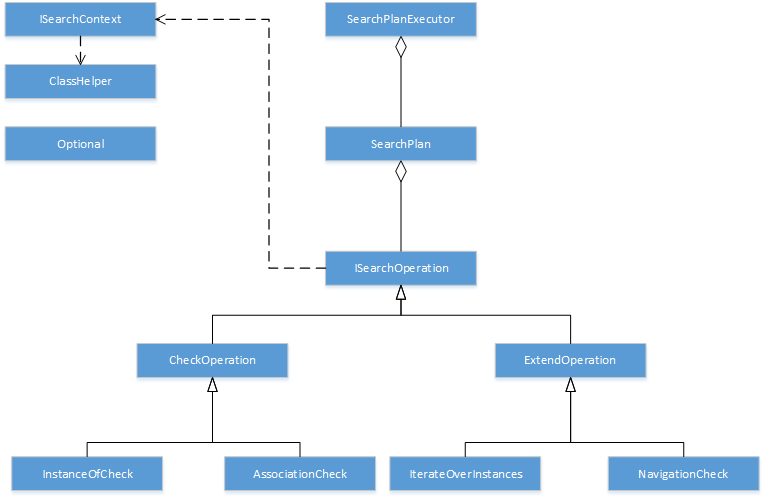
\includegraphics[width=150mm, keepaspectratio]{figures/runtime_diagram.png}
\caption{The runtime library}
\label{fig:runtime}
\end{figure}

The runtime library consists of three utility classes. The \emph{ISearchContext}
is the context of a search operation. It gives access to other utility class
instances parametrized correctly for the current search operations context. Such
utility class is the \emph{ClassHelper} which contains the dynamic instance
checking functionality described in section \sectref{InstanceChecking}. Another
utility class is \emph{Optional}, its purpose is detailed in
\sectref{MissingValueRepresentation}.

The rest of the library deals with the execution of a search plan. The central
piece of these classes is \emph{SearchPlan}. It contains an ordered list of
\emph{ISearchOperations}. An ISearchOperation can either be:

\begin{itemize}
  \item \emph{Check operation} - these type of operations receive one or more
  value and determines if a constraint is satisfied by them.
  \item \emph{Extend operation} - these operations receive zero or more values
  and based on those values calculates an additional value.
\end{itemize}

A check operation can either be an \emph{InstanceOfCheck} or an
\emph{AssociationCheck}. The InstanceOfCheck tests whether the provided value is
of the expected type. This is done as explained previously
(\sectref{InstanceChecking}). The AssociationCheck tests whether two values are
related through an association. This has two cases, if the association is [0..1]
multiplicity, this is a simple equality check, while if the association is
[0..*] then this is a list containment check.

Similarly to a check operation, the extend operation has two main types:
\emph{IterateOverInstances} and \emph{NavigateAssociation}. IterateOverInstances
simply assigns all instances of a class to a variable one by one.
NavigateAssociation gets a value and an association as a parameter and assigns
the instance or instances reached by navigating the association from the given
value to a variable.

The search plan is executed with the help of the \emph{SearchPlanExecutor}. The
search plan executor simply executes the search operations of a search plan and
returns if a match is found. This also provides an iterator with which a search
plan can be executed in a lazy manner.

\section{Generated code and API}\label{sect:generated_code_and_api}

The patterns defined with the \EIQ{} Pattern Language can be executed through
the usage of the generated classes. This chapter section goes into detail
explaining the generated classes.

The program supports two different approaches for executing the queries in the
generated code: \emph{runtime} based and \emph{iterator} based. The runtime
based fully utilizes the previously showcased local search runtime, assembles a
search plan and executes it. Meanwhile, the iterator based approach only uses a
few parts of the runtime and mostly uses built in language constructs.

\subsection{Runtime based}

This approach uses all the available runtime classes to generate a mostly easy
to understand human readable generated code where the search operations are
clearly visible. 

The generated artifacts for the runtime based approach can be seen on figure
\figref{runtime_gen}. The runtime based approach generates one header file per
query definition file and two header files for each pattern definition. 

\begin{figure}[!ht]
\centering
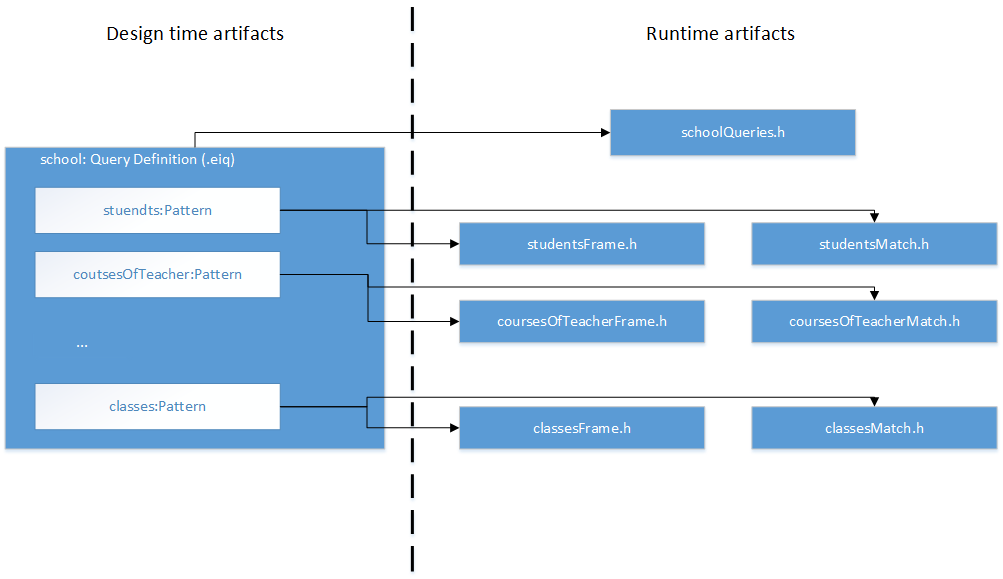
\includegraphics[width=130mm, keepaspectratio]{figures/runtime_gen_art.png}
\caption{The generated artifacts for the runtime based approach}
\label{fig:runtime_gen}
\end{figure}

The single central header file generated for a query definition file is named
after the original with the following pattern: \emph{<original .eiq name>Queries.h}.
Its function is to provide an API to call the defined patterns in multiple
ways:

\begin{itemize}
  \item \emph{get\_all\_<pattern>} - retrieves all matches for the defined pattern.
  \item \emph{get\_one\_<pattern>} - returns a single, arbitrary match for
  the defined pattern.
\end{itemize}

These methods also get generated with different parameter lists based on the
defined pattern bindings. More information about pattern bindings will be
explained in section \sectref{binding_variables}. In addition, it also contains
the initialization of the inheritance matrix which is generated from the
metamodel.

The two headers generated for a single pattern are representing a related
\emph{Frame} and a \emph{Match}. The frame is only used internally, it is a
simple struct containing all the variables used during the process of
executing the local search algorithm. The match represents a single match of the
pattern, it contains all the variables defined by the user as external variable
(defined in the patterns parameter list and not in the body), an equality
operator for the match and a hash function. The latter two are necessary to
check whether the match is unique. An additional difference between the two is
the type of the common external variables. A match always uses the strictest
determinable type from the type hierarchy, while a frame uses the least strict
type. Listing \listref{tos_pattern_spec} shows an example for this behavior. In
this pattern, course is defined as a \emph{SpecializationCourse} and as such,
the match will contain a \emph{SpecializationCourse} pointer. However, during
the query execution, navigating the courses association from \emph{School} will
yield regular \emph{Course}s. These have to be stored in the frame before the
type checking can be done and for this reason, the frame will hold
\emph{Course} pointers.

\begin{lstlisting}[frame=single,float=!ht,language=IQPL,
label=listing:tos_pattern_spec, caption=Specialization courses pattern] 
pattern specializationCoursesOfSchool(school, course) {
	School.courses(school, course);
	SpecializationCourse(course);
}
\end{lstlisting} 

To illustrate how the generated code is easy to understand, listing
\listref{tos_gen_runtime} shows the generated code for the
\emph{teachersOfSchool} pattern (reminder of the pattern in listing
\listref{tos_pattern_rem}). As seen in the code, the search plan is assembled
one operation at a time, while the operations are named in a way that it is easy
to understand what it will do. 

\begin{lstlisting}[frame=single,float=!ht,language=IQPL,
label=listing:tos_pattern_rem, caption=Teachers of school pattern as a
reminder] 
pattern teachersOfSchool(teacher, school) {
	School.teachers(school, teacher); 
}
\end{lstlisting}

In this example, the first operation is an instance iteration, where each
instance will be assigned to the first slot of the frame, and the iterated
instances are of the School class. The second operation navigates through a
School instance's teachers association and the found Teacher instances get
stored in the frames zeroth slot. Then as a third operation, the search checks if the
zeroth slot in the frame is of the Teacher type. This check seems unnecessary
and it is in this case, but if the School's teachers association pointed to a
parent type of Teacher, than the check would be required to filter out invalid
matches. This is a point in which the generated search plan could be further
optimized.

\begin{lstlisting}[frame=single,float=!ht,language=C++,
label=listing:tos_gen_runtime, caption=Segment of the generated code for
teachers of school]

SearchPlan< TeachersOfSchoolFrame> sp;
		
sp.add_operation(create_IterateOverInstances(&TeachersOfSchoolFrame::_1,
				School::type_id));
sp.add_operation(create_NavigateMultiAssociation(&TeachersOfSchoolFrame::_1,
				&TeachersOfSchoolFrame::_0,
				&School::teachers));
sp.add_operation(create_InstanceOfCheck(&TeachersOfSchoolFrame::_0,
				Teacher::type_id));

\end{lstlisting}


\subsection{Iterator based}

The iterator based approach is a much simpler approach than the runtime based
one, as it mostly uses built in language constructs and standard library
iterators. The main reason for this approach is that it reduses the dependency
on the runtime and it is slightly faster than the runtime based approach, but
the code readability is a lot worse and the generated code amount is much
larger. The generated artifacts are shown on figure \figref{iter_gen_art}.

\begin{figure}[!ht]
\centering
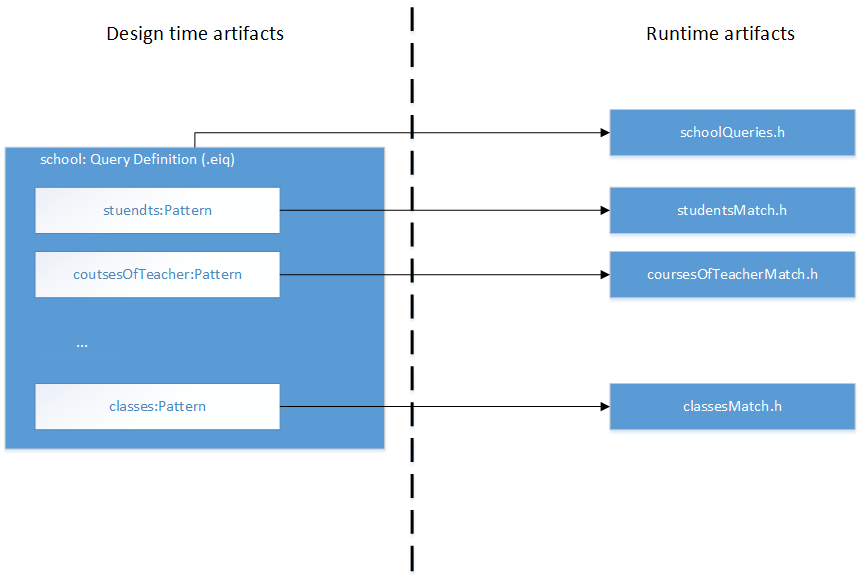
\includegraphics[width=120mm, keepaspectratio]{figures/iterator_gen_art.png}
\caption{The generated artifacts for the iterator based approach}
\label{fig:iter_gen_art}
\end{figure}

As the image shows, the generated artifacts are similar to the runtime based
approach. There is a single header file generated for each query definition
file and one-one additional header for each pattern. The difference is that it
is not necessary to generate the frames, as the variables the runtime stored in
the frame are held in local variables using this approach. This might suggest
that the generated code complexity got reduced, but the exact opposite is true
as listing \listref{tos_gen_iter} illustrates.

\begin{lstlisting}[frame=single,float=!ht,language=C++,
label=listing:tos_gen_iter, caption=Segment of the generated code for
teachers of school]

for(auto&& school : (::school::school::School::_instances)) {
	for(auto&& teacher : school->teachers) {
		if(_classHelper->is_super_type(teacher->get_type_id(), Teacher::type_id)) { 
			<assemble match> 
		}
	}
}

\end{lstlisting}

This code segment does exactly the same as the one shown for the runtime. In
this case, the code might even seem shorter, but as the queries grow larger the
code gets a lot more convoluted, for example when the search plan consists of
tens or even hundreds of steps, it gets hard to determine what the if statement
in the middle of the plan does, meanwhile in the case of the runtime based
approach, it will still be obvious as the method name itself tells what the
operation does. 

The above mentioned negatives of this approach are negligible, since the human
readability of a generated code is usually not important. For a release build,
it is always better to use this approach, as it is faster because there is no
need to check which operation is next from a search plan and the compiler can
generate more efficient bytecode since it is far easier to optimize this
version. In addition, the readability of this version could be improved through
annotating the code with comments describing which search operation gets
executed.

\subsection{Binding variables}\label{sect:binding_variables}

As previously mentioned, it is possible to bind variables of a pattern before
executing the query. This means that it is possible to predetermine the value of
a pattern variable, thus reducing the resulting matches to those that have the
predefined value in the specific variable. This is mostly useful if the query
can start from a predefined element of a model, significantly reducing the
pattern complexity.

The variable bindings have to be defined during query development time. The
generated code will adapt to the defined bindings and generate methods with the
specified parameters for a query. Listing \listref{pattern_binding} shows an
example of binding a parameter for a pattern.

\begin{lstlisting}[frame=single,float=!ht,language=IQPL,
label=listing:pattern_binding, caption=Binding of a parameter]

@Bind(parameters={teacher})
pattern classesOfTeacher(teacher, schoolClass) {
	find coursesOfTeacher(course, teacher);
	Course.schoolClass(course, schoolClass);
}

\end{lstlisting}

The parameter binding is done through the \emph{@Bind} annotation, where the
parameters have to be specified. It is possible to define multiple variables by
enumerating them using comma as a separator. The example binds the
\emph{classesOfTeacher} patterns \emph{teacher} parameter. That means a method
gets generated with a Teacher instance as a parameter which has to be specified.
